\documentclass[final]{fhnwreport}       %[mode] = draft or final
                                        %{class} = fhnwreport, article, 
                                        %          report, book, beamer, standalone
%%---Main Packages-----------------------------------------------------------------------
\usepackage[english, ngerman]{babel}	%Mul­tilin­gual sup­port for LaTeX
\usepackage[T1]{fontenc}				%Stan­dard pack­age for se­lect­ing font en­cod­ings
\usepackage[utf8]{inputenc}				%Ac­cept dif­fer­ent in­put en­cod­ings
\usepackage{lmodern}                    %The newer Font-Set
\usepackage{textcomp}					%LaTeX sup­port for the Text Com­pan­ion fonts
\usepackage{caption}					%Customising captions in floating environments
\usepackage{graphicx} 					%En­hanced sup­port for graph­ics
\usepackage{float}						%Im­proved in­ter­face for float­ing ob­jects
\usepackage{ifdraft}                    %Let you check if the doc is in draft mode
\usepackage{wrapfig}                    %Let wrap text around figures

%%---Useful Packages---------------------------------------------------------------------
\usepackage{color}						%Colour control for LaTeX documents
\usepackage[pdftex,dvipsnames]{xcolor}  %Driver-in­de­pen­dent color ex­ten­sions for LaTeX
\usepackage{csquotes}                   %Simpler quoting with \enquote{}
\usepackage{siunitx} 					%A com­pre­hen­sive (SI) units pack­age
\usepackage{listings}					%Type­set source code list­ings us­ing LaTeX
\usepackage[bottom]{footmisc}			%A range of foot­note op­tions
\usepackage{footnote}					%Im­prove on LaTeX's foot­note han­dling
\usepackage{verbatim}					%Reim­ple­men­ta­tion of and ex­ten­sions to LaTeX ver­ba­tim
\usepackage[textsize=footnotesize]{todonotes} %Mark­ing things to do in a LaTeX doc­u­ment
\usepackage{titling}					%Control over the typesetting of the \maketitle command

%%---Tikz Packages-----------------------------------------------------------------------
\usepackage{standalone}
\usepackage{tikz}
\usepackage{circuitikz}
\usetikzlibrary{arrows}
\usetikzlibrary{calc}
\usetikzlibrary{intersections}

%%---Math Packages-----------------------------------------------------------------------
\usepackage{amsmath}					%AMS math­e­mat­i­cal fa­cil­i­ties for LaTeX
\usepackage{amssymb}					%Type­set­ting symbols (AMS style)
%\usepackage{amstext}
%\usepackage{amsfonts}
%\usepackage{breqn}
\usepackage{array}						%Ex­tend­ing the ar­ray and tab­u­lar en­vi­ron­ments
\usepackage{amsthm}					%Type­set­ting the­o­rems (AMS style)

%%---Table Packages----------------------------------------------------------------------
\usepackage{booktabs}
%\usepackage{vcell}
\usepackage{tabularx}					%Tab­u­lars with ad­justable-width columns
%\usepackage{longtable}
\usepackage{multirow}					%Create tab­u­lar cells span­ning mul­ti­ple rows
\usepackage{makecell}
\usepackage{multicol}					%In­ter­mix sin­gle and mul­ti­ple columns
\usepackage[normalem]{ulem}
\useunder{\uline}{\ul}{}

%%---PDF / Figure Packages---------------------------------------------------------------
\usepackage{pdfpages}					%In­clude PDF doc­u­ments in LaTeX
\usepackage{pdflscape}					%Make land­scape pages dis­play as land­scape
\usepackage{subfig}					    %Fig­ures di­vided into sub­fig­ures

%%---Other Packages----------------------------------------------------------------------
%\usepackage{xargs}                     %De­fine com­mands with many op­tional ar­gu­ments

\lstset{
	aboveskip=1ex,
	backgroundcolor=\color{gray!25},
	basicstyle=\small\ttfamily,
	belowskip=1ex,
	breaklines=true,
	columns=fullflexible,
	framerule=0pt,
	framexrightmargin=0em,
	framexleftmargin=0em,
	numbers=left,
	numberstyle=\footnotesize\sffamily,
	tabsize=2
}

\lstdefinestyle{DOS}
{
	backgroundcolor=\color{black},
	basicstyle=\scriptsize\color{white}\ttfamily
}


%%---Bibliography------------------------------------------------------------------------
\usepackage[style=ieee,urldate=comp,backend=biber]{biblatex}
\addbibresource{literature/bibliography.bib}

%%---Main Settings-----------------------------------------------------------------------
\graphicspath{{./graphics/}}			%Defines the graphicspath
\geometry{twoside=false}				    %twoside=false disables the "bookstyle"
\setlength{\marginparwidth}{2cm}
\overfullrule=5em						%Creates a black rule if text goes over the margins => debugging




%%---User Definitions--------------------------------------------------------------------
%%Tabel-Definitions: (requires \usepackage{tabularx})
\newcolumntype{L}[1]{>{\raggedright\arraybackslash}p{#1}}    %column-width and alignment
\newcolumntype{C}[1]{>{\centering\arraybackslash}p{#1}}
\newcolumntype{R}[1]{>{\raggedleft\arraybackslash}p{#1}}

%%---Optional Package Settings-----------------------------------------------------------
%Listings-Settings: (requires \usepackage{listings}) => Example with Matlab Code
%\lstset{language=Matlab,%
%    basicstyle=\footnotesize\ttfamily,
%    breaklines=false,%
%    morekeywords={switch, case, otherwise},
%    keywordstyle=\color{Blue},%
%    tabsize=2,
%    %morekeywords=[2]{1}, keywordstyle=[2]{\color{black}},
%    identifierstyle=\color{Black},%
%    stringstyle=\color{Purple},
%    commentstyle=\color{Green},%
%    showstringspaces=false,%without this there will be a symbol in the places where there is a space
%    numbers=left,%
%    numberstyle={\tiny \color{black}},% size of the numbers
%    numbersep=9pt, % this defines how far the numbers are from the text
%    %emph=[1]{word1, word2,...},emphstyle=[1]\color{red}
%}							

%Hurenkinder und Schusterjungen verhindern (kein Scherz, Google es)
\clubpenalty10000
\widowpenalty10000
\displaywidowpenalty=10000	


%%---Costum Packages Bachelor Thesis-------------------------------------------
\usepackage{diagbox}

\usepackage{hyperref}
\hypersetup{
    colorlinks=true,
    linkcolor=black,
    filecolor=black,       
    urlcolor=blue,
    citecolor=black,
}			                %loads all packages, definitions and settings
\addbibresource{literature/bibliography.bib}							
\title{Pflichtenheft}  		        %Project Title
\author{Anklin, Bobst, Horath}      				    %Document Type => Technical Report, ...
\date{\today}          				   %Place and Date

\begin{document}

%%---TITLEPAGE---------------------------------------------------------------------------------
\thispagestyle{empty}
%	\ohead{\includegraphics[scale=0.5]{Bilder/Logo_FHNW.jpg}}
	\begin{figure}
		 \vspace*{-\topskip}\vspace*{-\headsep}
		
\includegraphics[scale=1]{graphics/fhnw_ht_logo_de.pdf}
	\end{figure}
	\begin{center}
		\vspace*{2cm}
		{\huge{\textbf{\thetitle}}}\\
		\vspace*{1cm}
		
		{\huge{Bluetooth-Mesh Plattform für IoT Anwendungen}}\\
		\vspace*{0.5cm}
		
		{\scshape\Large Projekt 5 - \theauthor \\} \Large{\today}
		\vfill
		
		
		\begin{normalsize}
			{\begin{tabbing}
						
					\textbf{Fachcoach:} \hspace{6cm}\= Matthias Meier\\
					\>Manuel Di Cerbo\\
					
					\\[0.4cm]
					
					\textbf{Team:} \>Raffael Anklin \\ \>Robin Bobst \\ \>Cyrill Horath
					\\[0.8cm]
					\textbf{Studiengang:} \>Elektro- und Informationstechnik
					\\[0.8cm]	\textbf{Semester:} \>Herbstsemester 2019
			\end{tabbing}}
		\end{normalsize}
		\vfill
	\end{center}
\clearpage


%%---TABLE OF CONTENTS-------------------------------------------------------------------
\pagenumbering{Roman}		
\selectlanguage{ngerman}				%ngerman or english
\tableofcontents
\clearpage

%%---TEXT--------------------------------------------------------------------------------
\pagenumbering{arabic}
	\clearpage
\section{Übersicht}\label{sec:Uebersicht}

Das vorliegende Dokument stellt das Pflichtenheft der Bachelorthesen von Raffael Anklin, Robin Bobst und Cyrill Horath an der Fachhochschule Nordwestschweiz Brugg-Windisch im Studiengang Elektro- und Informationstechnik dar. 
Im kommenden, ersten Kapitel soll eine Übersicht über die Ausgangslage sowie das Ziel dieser Arbeit gegeben werden und somit die Rahmenbedingungen abgesteckt werden. Weiter werden die Lösungskonzepte \ref{sec:Loesungskonzept} sowie die Projektziele und Lieferobjekte \ref{sec:ProjektzieleundLieferobjekte} definiert. Abschliessend soll auch noch das Projektmanagement \ref{sec:Projektmanagement} thematisiert werden. 

\subsection{Ausgangslage}\label{subsec:Ausgangslage}

Unter den standardisierten Low Power Mesh Netzwerk Protokollen im
freien GHz ISM-Band konkurrenzieren sich derzeit vorrangig Bluetooth Mesh, Zigbee sowie Thread.
Bezüglich MAC und Physical Layer basieren Zigbee und Thread auf IEEE 802.15.4 wogegen Bluetooth Mesh auf Bluetooth Low Energy (BLE)
basiert.
Jedes dieser Netzwerkprotokolle hat gewisse Vorzüge: Bluetooth Mesh, dass BLE mittlerweile von jedem Smartphone und Notebook unterstützt wird, Thread aufgrund seiner IPv6 Basis und damit einfachem Übergang ins Internet sowie Zigbee aufgrund seiner etablierten Verbreitung im Smart-Lampenbereich durch Philips, IKEA und Osram.
Hauptproblem aller drei Mesh Netzwerkprotokolle ist nebst physikalisch und distanzbedingter Absorption und Reflexion die Störbeeinflussung durch WLAN (WiFi) und andere Netzwerke im GHz Frequenzbereich.

Im Vorprojekt im Rahmen des P5 mit dem Namen \textit{Bluetooth-Mesh Plattform für IoT Anwendungen} zu dieser Arbeit, wurde das Bluetooth-Mesh Protokoll bereits vertieft betrachtet und dessen Vor- und Nachteile aufgezeigt. Basierend auf diesen Erkenntnissen und Erfahrungen und der oben beschriebenen Thematik soll das Bluetooth-Mesh Protokoll mit den Alternativen Thread sowie Zigbee verglichen werden.

\subsection{Ziel der Arbeit}\label{subsec:ZielderArbeit}

In der vorliegenden Arbeit soll zuerst ein praxistaugliches, einheitliches Testframework für alle drei Mesh Netzwerke erstellt werden, wonach die Tauglichkeit aller drei Mesh Netzwerke unter realitätsnahen Bedingungen ermittelt und verglichen werden soll.
Zwecks besserer Vergleichbarkeit sollen alle drei Testnetze das gleiche Radio-Interface als Grundlage verwenden. Aufgrund der guten
Unterstützung aller drei Mesh Protokolle als auch dem im vergangenen P5 gesammelten Wissens, sollen hierfür die nRF52840 SoCs der Firma Nordic eingesetzt werden. Die zu erstellende Testinfrastruktur soll aus den drei folgenden Teilen bestehen:

\begin{itemize}
 	\item Punkt-Punkt Testinfrastrukturen auf MAC-Ebene
 	\item Test Mesh Netzwerke für BT Mesh, Zigbee und Thread
 	\item Steuer- und Auswertesoftware
\end{itemize}

Die genauen Anforderungen an die Testumgebung sind einerseits in der Aufgabenstellung im Anhang \ref{app:Aufgabenstellung} aufgeführt und andererseits werden sie anhand der Projektziele \ref{sec:ProjektzieleundLieferobjekte} definiert.









	
\subsection{Ausgangslage}\label{subsec:Ausgangslage}

Die Bluetooth Technik wurde im Jahr 1998 von der "Bluetooth Special Interest Group" (SIG) als Industriestandart für Datenübertragung herausgebracht. Ursprünglich wurde das Funkverfahren jedoch von Jaap Hartsen und Sven Mattisson für die Firma Ericsson entwickelt. Der Hauptzweck dieser Methode zur Datenübermittlung war das Ersetzen von Kabelverbindungen von Mobiltelefone, Peripheriegeräte oder Computer. Der Name Bluetooth oder auf Deutsch Blauzahn kommt vom dänischen König Harald Blauzahn. Diesem König gelang es die verfeindeten Länder Dänemark und Norwegen dank seiner Kommunikationsfreudigkeit zu vereinen. Da die skandinavischen Firmen Nokia und Ericsson viel Aufwand in die Bluetooth Technologie gesteckt haben, wurde dieser Name sowie die Runen H (Harald) und B (Blauzahn) für das Logo übernommen.\cite{michna_entwicklungsgeschichte_2019} Seit dem Start von Bluetooth gab es eine Vielzahl von Versionen, die von mehreren Firmen ständig weiterentwickelt werden. Im Dezember 2009 wurde von der SIG die Version 4.0 Smart vorgestellt. Mit dieser Version von Bluetooth war es möglich kleine und sparsame Geräte wie z.B. smarte Uhren, Brillen oder sogar Ringe herzustellen.\cite{bluetooth_sig_our_2019} Ab dem Jahre 2017 ist es möglich Bluetooth Komponenten in einem Mesh-Netzwerk zu konfigurieren.\cite{eckstein_neue_2019} Dieses Netzwerk basiert auf einem "many-to-many pairing system" d.h. jeder Teilnehmer ist mit den anderen Teilnehmern verbunden. Dieses dezentralisierte System hat den Vorteil, dass es kein Master Element benötigt. Fällt ein Teilnehmer aus besteht das Netzwerk trotzdem weiter.\cite{woolley_intro_2017} Genau hier soll das Projekt 5 ansetzten. Da die Programmierung eines Mesh-Netzwerkes sehr kompliziert ist, wird dafür eine "'Open Source Software"' geschrieben, die es ermöglicht ein Netzwerk vereinfacht aufzubauen und zu konfigurieren.










	\clearpage
\subsection{Projektziele}\label{subsec:Projektziele}
In den beiden Tabellen \ref{tab:Pflichtziele} und \ref{tab:Wunschziele} sind die Pflicht- resp. Wunschziele für dieses Projekt festgehalten.

\begin{table}[H]
\begin{tabular}{ | C{0.9cm} | p{3.3cm} | p{10cm} |}
	\hline
	\multicolumn{3}{|l|}{\textbf{Pflichtziele}}\\ \hline
\textbf{Nr.}& \textbf{Ziel}& \textbf{Beschrieb}\\ \hline

P1 & Bluetooth-Mesh-Netzwerk & Eine variable Anzahl an BLE-Nodes bauen ein Mesh-Netzwerk auf um darin Datenaustausch zu ermöglichen.\\ \hline

P2 & UPN & Der Universal-Peripheral-Node kann je nach Einsatz als Sensor oder Aktor konfiguriert und bestückt werden.\\ \hline

P3 & Low Power & Die UPN sind bezüglich Hardware und Software energiesparend konzipiert um sie autonom betreiben zu können.\\ \hline

P4 & Security & Das Mesh-Netzwerk ist gegen unerlaubten Zugriff und sonstigen Angriffen geschützt.\\ \hline

P5 & Netzunabhängig & Durch Versorgung mittels Batterie und Energy-Harvesting können die UPN komplett netzunabhängig betrieben werden.\\ \hline

P6 & Energy-Harvesting & Für die Versorgung der UPN werden verschiedene Varianten für das Energy-Harvesting entwickelt. Das Ergebnis wird eine Variantenstudie sein.\\ \hline

P7 & Gateway & Zur Konfiguration des Bluetooth-Mesh-Netzwerks steht ein Gateway basierend auf Standard Hardware (Raspberry-Pi + nRF52840 USB Dongle o.ä.) zur Verfügung.\\ \hline
    
P8 & LAN/WLAN & Für die Integration in TCP/IP basierte Systeme bietet der Gateway eine entsprechende Schnittstelle.\\ \hline

P9 & CLI & Mittels Command-Line-Interface kann das Mesh-Netzwerk verwaltet werden.\\ \hline

\end{tabular}\\
\caption{Pflichtziele}
\label{tab:Pflichtziele}
\end{table}


\begin{table}[H]
\begin{tabular}{ | C{0.9cm} | p{3.3cm} | p{10cm} |}
	\hline
	\multicolumn{3}{|l|}{\textbf{Wunschziele}}\\ \hline
\textbf{Nr.}& \textbf{Ziel}& \textbf{Beschrieb}\\ \hline
    	 
    
W1 & UPN Konfiguration via Mesh & Einstellungen des UPN können via Mesh Netzwerk angepasst werden und somit z.B. die Peripheriekonfiguration verändert werden.\\ \hline

W2 & Firmwareupgrade via Mesh & Die Firmware der UPN wird via Mesh-Netzwerk aktualisiert. \\ \hline

W3 & BLR und BLE & Bluetooth Long Range (BLR) und Bluetooth Low Energy (BLE) ergänzen das Bluetooth Mesh um die Reichweite zu vergrössern oder den Energieverbrauch nochmals zu vermindern. \\ \hline

W4 & Dedizierte Hardware UPN & Das UPN ist als dedizierte Hardware realisiert und somit einsatzbereit. \\ \hline

W5 & Datenschnittstelle & Mittels passender Datenschnittstelle auf dem Gateway können Fremdsysteme wie Apple Homekit, Google Home oder KNX angebunden werden.\\ \hline

W6 & Datenschnittstelle ohne Zwischenspeicherung & Damit keine Daten auf dem Gateway zwischen gespeichert werden müssen können die Nodes mittels verbindungslosem Protokoll (MQTT, CoAP, usw.) direkt aus dem Mesh Netzwerk mit einem Fremdsystemen kommunizieren. \\ \hline

W7 & HMI & Ein Human-Machine-Interface in Form einer Webapplikation unterstützt den User bei der Konfiguration des Mesh-Netzwerks und ermöglicht die Anbindung an Fremdsysteme. \\ \hline

W8 & Dedizierte Gateway Hardware & Der Gateway ist auf einer dedizierten Hardware umgesetzt. \\ \hline

W9 & Onboard Bluetooth & Da der Raspberry-Pi 4 bereits ein Bluetooh 5 Chip besitzt soll direkt dieser verwendet werden anstelle eines angeschlossenen Dongles. \\ \hline

W10 & Mobiltelefon & Anstelle oder ergänzend zum Gateways kann ein Mobiltelefon ins Mesh-Netzwerk eingebunden werden um Konfigurationen vorzunehmen oder Daten aus zu lesen. \\ \hline

W11 & GSM/LTE & Für Feldanwendungen besitzt der Gateway ein GSM/LTE Modul. \\ \hline

W12 & Versuchsaufbau Energy-Harvesting & Erfolg versprechende Energy-Harvesting-Systeme werden in einem Versuchsaufbau auf deren Tauglichkeit weiter geprüft. \\ \hline


\end{tabular}\\
\caption{Wunschziele}
\label{tab:Wunschziele}
\end{table}


















	\clearpage
\subsection{Lieferobjekte}\label{subsec:Lieferobjekte}
Zusätzlich zu den Projektzielen, folgen in diesem Kapitel die Lieferobjekte  mit dem jeweiligen Datum. In der Tabelle \ref{tbl:Lieferobjekte} sind diese  aufgelistet.  


\begin{table}[H]
     \centering
\begin{tabular}{|c|c|l|}\hline
   \textbf{Nr.} & \textbf{Datum} & \textbf{Lieferobjekt} \\ \hline
   
   1 & 07.10.2019 & Abgabe Pflichtenheft, 1. Version\\ \hline
   2 & 14.10.2019 & Abgabe Pflichtenheft, definitive Version\\ \hline
   3 & 13.01.2020 & Projektpräsentation \\ \hline
   4 & 13.01.2020 & Abgabe Fachbericht \\ \hline
   5 & 13.01.2020 & Abgabe Testaufbau Mesh-Netzwerk \\ \hline
   
   
   
 \end{tabular}
     \caption{Lieferobjekte}
     \label{tbl:Lieferobjekte}
\end{table}










\pagebreak

\clearpage
\section{Lösungskonzept}\label{sec:Loesungskonzept}
Zur Messung und Auswertung der Mesh-Netzwerke dient ein Testframework wie es in Abbildung \ref{fig:KonzeptschemaTestframework} schematisch dargestellt ist.

\begin{figure}[H]
	\centering
	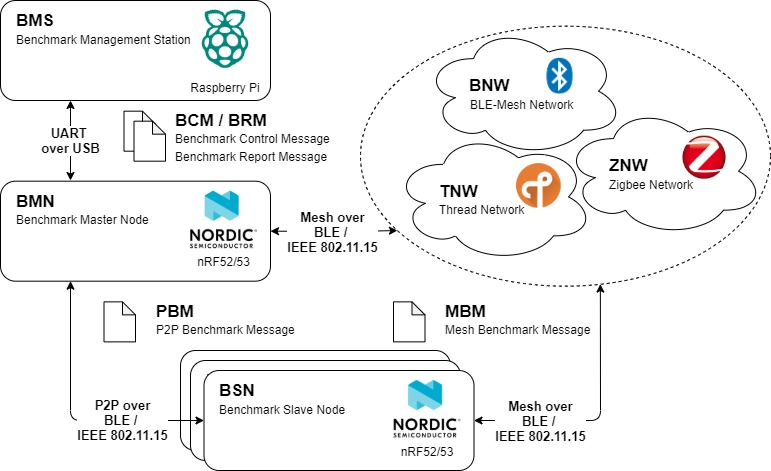
\includegraphics[width=1.0\textwidth]{Konzept_Testframework.jpg}
	\caption{Konzeptschema Testframework}\label{fig:KonzeptschemaTestframework}
\end{figure}


Das Testframework besteht aus folgenden physikalisch getrennten Teilsystemen:

\begin{itemize}
	\item \textbf{BMS} Benchmark Management Station \\ 
	Dient zur Verwaltung und Konfiguration des Testframeworks. Beinhaltet einen Webserver um dem Endanwender die Bedienung zu ermöglichen. Realisiert wird die BMS durch einen \textit{Raspberry Pi 4 Model B}. Als Webserver wird das Python-Framework \textit{Django} eingesetzt. 
	\item \textbf{BMN} Benchmark Master Node \\ 
	Dient als Zugangspunkt der BMS für die im Testframework gefahrenen Tests und lässt sich über eine Serielle Schnittstelle ansprechen. In der Aufgabenstellung \ref{app:Aufgabenstellung} wird der BMN als Master bezeichnet. Realisiert wird der BMN über einen nRF52840 oder nRF5340 von \textit{Nordic}. 
	\item \textbf{BSN} Benchmark Slave Node \\ 
	Dient als Zugriffspunkt der im Testframework gefahrenen Tests und kann frei in der Testumgebung platziert werden. Daher muss die Energieversorgung über einen Akku oder Batterie erfolgen. In der Aufgabenstellung  \ref{app:Aufgabenstellung} wird von einem Slave gesprochen. Realisiert wird der BSN über einen nRF52840 oder nRF5340 von \textit{Nordic}.
\end{itemize}

Die logischen Komponenten des Testframeworks lassen sich wie folgt aufteilen:

\begin{itemize}
	\item \textbf{BCM} Benchmark Control Message \\ 
	Beschreibt Nachrichten welche zur Steuerung eines Benchmarks dienen. Dies sind zum Beispiel Konfigurations-, Start- oder Stop-Befehle. Werden von der BMS initiiert und gelangen über eine USB-UART Verbindung zum BMN. 
	\item \textbf{BRM} Benchmark Report Message \\ 
	Beschreibt Nachrichten welche den Status oder die Ergebnisse eines Benchmarks zurückmelden. Werden vom BMN initiiert und gelangen über eine USB-UART Verbindung zur BMS.
	\item \textbf{PBM} P2P Benchmark Message \\ 
	Nachrichten welche während der Durchführung eines Benchmarks versendet werden. Dies sind zum Beispiel Ping-Anfragen zur Latenzzeitmessung. Sie ermöglichen den Datenaustausch zwischen zwei Teilnehmern auf MAC-Ebene. 
	\item \textbf{MBM} Mesh Benchmark Message \\ 
	Nachrichten welche während der Durchführung eines Benchmarks versendet werden. Dies sind zum Beispiel Ping-Anfragen zur Latenzzeitmessung. Sie ermöglichen den Datenaustausch über ein Mesh-Netzwerk auf Applikations-Ebene. 
\end{itemize}

\subsection{Punkt zu Punkt Testinfrastruktur}\label{subsec:PunktzuPunktTestinfrastruktur}

Der Punkt zu Punkt Benchmark (P2P) soll unabhängig vom Mesh-Protokoll stattfinden. Damit soll es möglich sein die beiden MAC-Ebenen \textit{BLE} und \textit{IEEE802.11.15} zu vergleichen. Der nRF52840 sowie nRF5340 unterstützen das Arbeiten auf der MAC-Schicht. Zur Realisierung wird ein bereits bestehendes Beispiel (Radio-Example) aus der nRF Connect SDK genutzt.


\subsection{Test Mesh Netzwerke}\label{subsec:TestMeshNetzwerke}

Der Mesh-Benchmark soll die verschiedenen Mesh-Netzwerke möglichst identisch ausmessen. Dazu dient bei allen Mesh-Netzwerken die Applikations-Schicht. Ein Mesh Netzwerk wird zwischen dem BMN und den BSN aufgebaut. Dazu werden die einzelnen Nodes über die BMS mit der entsprechenden Firmware geladen und anschliessend im Raum verteilt. Das Laden ist zu Beginn über eine Kabelverbindung (UART) vorgesehen. Zu einem späteren Zeitpunkt soll dies drahtlos mithilfe eines Bootloaders möglich gemacht werden. 

\subsubsection{Bluetooth Mesh}\label{subsubsection:Bluetooth Mesh}

Die BLE-Mesh Firmware der Nodes werden aus Beispielen der nRF Connect SDK und Zephyr abgeleitet. Das Mesh-Demo Beispiel erlaubt es die essentiellen Netzwerk Parameter fix vorzugeben. Dadurch müssen die Nodes nicht mehr Provisioniert werden und sind sofort einsatzbereit.

\newpage
\subsubsection{Thread}\label{subsubsection:Thread} 
Die Abbildung \ref{fig:ThreadKonzept} zeigt das Framework des Openthread Netzwerkes auf. Die BMS kommuniziert via UART mit dem wpantund Protokoll von Google. Die Daten zum NCP, welcher auf dem BMN realisiert wird, werden mit Hilfe von Spinel übertragen. Der BMN sendet die erhaltenen Daten danach in das Thread Netzwerk.

\begin{figure}[H]
	\centering
	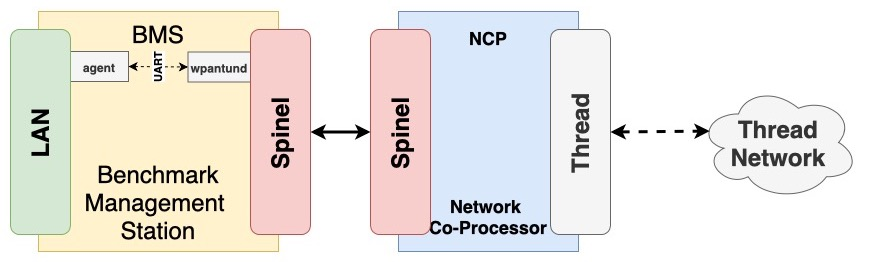
\includegraphics[width=1.0\textwidth]{Thread-Konzept.jpg}
	\caption{Konzept OpenThread Framework}\label{fig:ThreadKonzept}
\end{figure}



\subsubsection{Zigbee}\label{subsubsection:Zigbee}
Das Zigbee Test Mesh Netzwerk wird mithilfe der \textit{nRF SDK for Thread and Zigbee} eingerichtet und für die Messungen vorbereitet. Der BMN wird dabei als Zigbee Coordinator und gleichzeitig als Zigbee Router eingesetzt. Die BSN können wieder als Router oder aber als Zigbee End Device betrieben werden.


\subsection{Steuer und Auswertesoftware}\label{subsec:SteuerundAuswertesoftware}
Die Steuerung des Testframeworks erfolgt über eine Weboberfläche. Diese wird von der BMS mittels WLAN auf den Benutzergeräten zur Anzeige gebracht. Als Webserver dient das Python-Framework \textit{Django}. Zur Steuerung der Benchmarks dienen Schrittketten, welche mit der Firmware auf dem BMN kommunizieren. Als letzter Schritt eines Benchmarks werden die Ergebnisse geloggt, nachbearbeitet und wiederum zur Anzeige gebracht.


\pagebreak

\clearpage
\section{Hardware}\label{sec:Hardware}
In diesem Kapitel wird die Hardware vom \textit{Gateway Interface System}, dem \textit{Universal Peripheral Node}, dem \textit{Energy Harvesting System} und dem \textit{Power Storage System} beschrieben. 


\subsection{Bluetooth Mesh Node (BMN)}\label{subsec:BMN}
Im Bluetooth Mesh Protokoll gibt es zwei verschiedene  Geräte, ein \textit{"'unprovisioned device"'} und einen \textit{"'node"'}. Das \textit{"'unprovisioned device"'}  ist ein Teilnehmer, der für das Mesh Netzwerk unbekannt ist und deshalb keine Rechte besitzt. Wird dieses Gerät nun in das Netzwerk aufgenommen, so wird das \textit{"'unprovisioned device"'}  zu einem \textit{"'node"'}. Dieses vorgehen nennt sich \textit{"'provisioning"'}.\cite{afaneh_ultimate_2018} Die Hardware für den \textit{"'node"'} besteht bei allen Geräten aus dem gleichen SoC. Der nRF52840 von Nordic Semiconductor eignet sich aus folgenden Gründen perfekt für diese Anwendung. Die \textit{"'nodes"'} dürfen, um eine lange Laufzeit zu garantieren, sehr wenig elektrische Leistung beziehen. Der nRF52840 benötigt im Ruhemodus nur wenige $[\mu A]$. Ein weiterer Grund ist die sehr gute Dokumentation der Software von Nordic Semiconductor. Die gesamte Software ist im Infocenter erhältlich und frei zugänglich. Weitere Vorteile befinden sich in der Tabelle \ref{tbl:Vorteilte_nRF52}:\cite{nordic_semiconductor_nrf52840_2019} \\

\begin{table}[h]
	\begin{tabular}{ll}
		\multicolumn{2}{l}{{\ul \textbf{Vorteile des nRF52840}}}       \\
		Bluetooth 5                          											   & -95 dBm Sensivität      \\
		Multiprotokoll (Thread, Zigbee, usw) 						   & +8 dBm Ausgangsleistung \\
		Geringer Stromverbrauch  (wenige $[\mu A]$)      	& USB 2.0                 \\
		12bit ADC                            												& NFC                     \\
		1 MB flash und 256kB RAM Speicher    						& ARM M4F Cortex         
	\end{tabular}
	\caption{Vorteile des nRF52840}
	\label{tbl:Vorteilte_nRF52}
\end{table}


\begin{figure}[h]
	\centering
	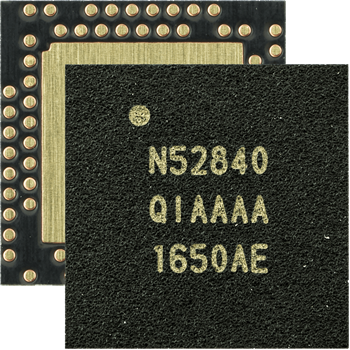
\includegraphics[scale=0.5,angle=0]{nRF52840.png}
	\caption{nRF52840 SoC \cite{nordic_semiconductor_nrf52840-qiaa.png_2019}}
	\label{img:nRF52840}
\end{figure} 

\subsection{Gateway Interface System (GIS)}\label{subsec:Gateway}
Der Bluetooth-Mesh-Gateway soll die Plattform gegenüber Fremdsystemen öffnen und damit die Schnittstelle zu IOT Anwendungen (Internet of Things) bilden. Damit die Plattform einfach zu betreiben ist, wird beim Gateway in erster Linie auf den Einplatinen-Computer Raspberry-Pi 4 (siehe Abschnitt \ref{img:raspberryPi4}) gesetzt. Andere Einplatinen-Computer wären ebenfalls denkbar wobei die Raspberry-Pi-Plattform bereits sehr weit verbreitet ist und somit oft bereits verfügbar ist.

Der Raspberry-Pi 4 besitzt nebst Ethernet und WLAN Schnittstellen sowie USB 3 Ports auch von Grund auf mit einem Bluetooth 5 Modul ausgestattet. So könnte er direkt ins Bluetooth-Mesh-Netzwerk integriert werden. Um jedoch die volle Integration zu erreichen, wird in erster Linie der oben erwähnte nRF52840 (siehe Abschnitt \ref{subsec:BMN}) in Form eines Dongle-Development-Boards \ref{img:nRF52840USBDongle} eingesetzt. Via serieller Schnittstelle wird dieser mit dem Raspberry-Pi 4 verbunden.

Als Ergänzung oder Alternative zum Gateway soll beispielsweise ein Mobiltelefon welches ein Bluetooth Modul besitzt ins Mesh Netzwerk integriert werden können. Darüber sollen dann Konfigurationen sowie die Ein- und Ausgabe von Parametern und Daten möglich sein. 


\begin{figure}[h]
	\centering
	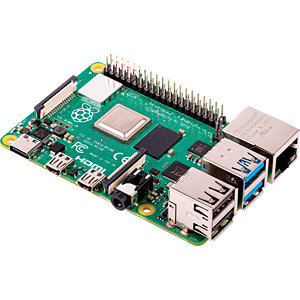
\includegraphics[scale=0.7,angle=0]{RASP_PI_4_B.jpg}
	\caption{Raspberry-Pi 4 \cite{reichelt_elektronik_gmbh_&_co_kg_rasp_nodate}}
	\label{img:raspberryPi4}
\end{figure} 

\begin{figure}[h]
	\centering
	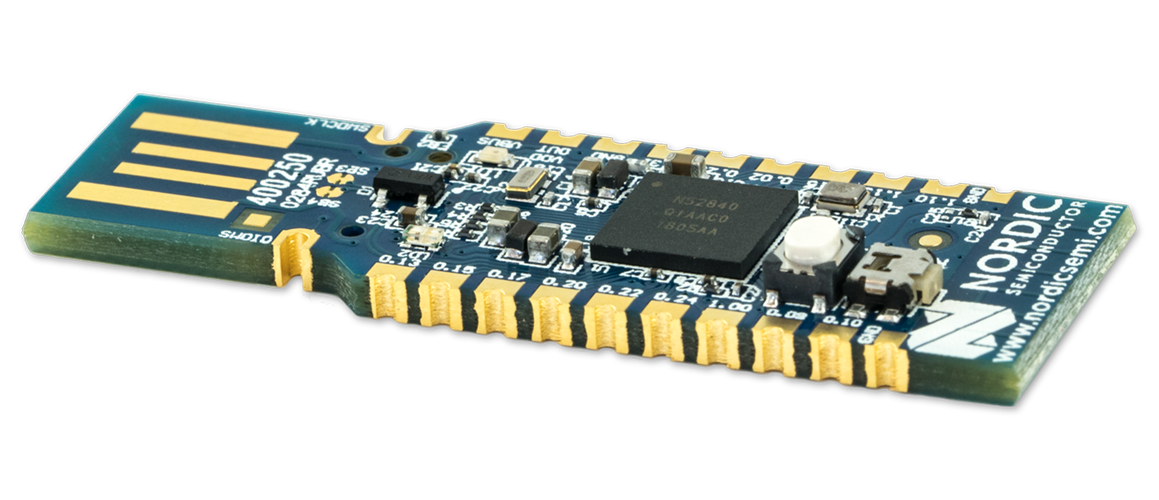
\includegraphics[scale=0.2,angle=0]{nRF52840_Dongle.png}
	\caption{nRF52840 USB Dongle \cite{nordic_semiconductor_nrf52840-dongle-promo.png_2019}}
	\label{img:nRF52840USBDongle}
\end{figure} 


\subsection{Energy Harvesting System (EHS)}\label{subsec:EHS}

Das \textit{EHS} beinhaltet unterschiedlichen Methoden um Energie aus der Umgebung aufzufangen. Diese sind in der folgenden Tabelle mit den wichtigsten Kenndaten aufgefasst. 

\begin{figure}[h]
	\centering
	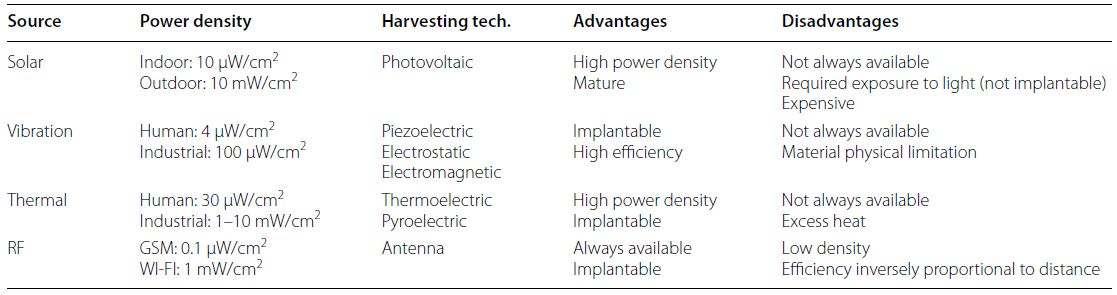
\includegraphics[scale=0.50,angle=0]{Tabelle_Energyharvesting_Sources.jpg}
	\caption{Tabelle Umgebungsenergie \cite{tran_rf_2017}}
	\label{img:Tabelle_Energyharvesting_Sources}
\end{figure} 

Durch Berechnungen, Simulationen und Testaufbauten soll gezeigt werden, welche Methode sich als genügend ertragreich für unser System erweist. Dafür muss der Energiebedarf des Systems gemessen werden. Die Messungen erfolgen unter verschiedenen Konfigurationen. Mithilfe der Ergebnisse soll es möglich sein, die optimale Konfiguration situationsbedingt zu wählen.



\subsection{Power Storage System (PSS)}\label{subsec:PSS}
Das \textit{PSS} ist für die Energiespeicherung zuständig. Untersucht wird die Speicherung der gewonnen Energie aus dem \textit{EHS} mithilfe Sekundärer Zellen (Akkus) oder mit \textit{Supercaps}. Der Einsatz eines Tiefendladungsschutzes ist bei verwenden der sekundären Zellen angedacht. Zusätzlich soll die Versorgung aus primären Zellen untersucht werden. Mithilfe der Ergebnisse soll es möglich sein, die optimale Konfiguration situationsbedingt zu wählen.   

 

\pagebreak

\clearpage
\section{Software}\label{sec:Software}
Das Kapitel Software befasst sich mit der Programmierung des Mikrocontroller \textit{nRF52840} sowie des \textit{GIS}.

\subsection{Software BMN}\label{subsec:SoftwareBMN}
Die Software auf dem \textit{BMN} (siehe Abschnitt \ref{subsec:BMN}) wird mit Hilfe der folgenden \textit{SDKs} von \textit{Nordic Semiconductor} entwickelt:

 \begin{itemize} 
	\item \textit{nRF5 SDK}\cite{nordic_semiconductor_nrf5_2019}
	\item \textit{nRF5 SDK for Mesh}\cite{nordic_semiconductor_nrf5_2019-1}
	\item \textit{Zephyr}\cite{zephyr_project_zephyr_2019}
\end{itemize}

Diese \textit{SDKs} enthalten eine sehr gut dokumentierte Bibliothek, die für den Quellcode des \textit{BMN} benötigt werden.


\subsection{Software GIS}\label{subsec:SoftwareGIS}
Mit dem Ziel den Gateway Open Source und Open Hardware zu realisieren, soll eine einfache Linux-Distribution eingesetzt werden. Beim Raspberry-Pi 4 (siehe Abschnitt \ref{img:raspberryPi4}) eignet sich dafür besonders das Debian basierende Betriebssystem Raspbian da es eigens für die Raspberry-Pi Familie entwickelt wurde.

Basierend auf dieser Oberfläche können nun Anbindungen an Fremdsysteme wie \textit{Apple Homekit} oder \textit{KNX} mit den passenden Software Bausteinen realisiert werden. Welche Bausteine dies sein werden ist Teil der Umsetzung für eine spezifische Anwendung welche noch nicht festgelegt ist. Daher wird in erster Linie mit einfachen Sprachen wie beispielsweise \textit{Node.js} oder \textit{Python} eine Ein- und Ausgabe von Daten oder Befehlen umgesetzt. 

\subsection{Human Machine Interface (HMI)}\label{subsec:HMI_SW}
Das \textit{HMI} wird kein primäres Ziel sein. Angedacht wird ein einfaches \textit{Webinterface} zur Konfiguration des \textit{Mesh-Netzwerkes}.

\subsection{Security}\label{subsec:Security}
Der Bluetooth-Mesh-Standart von (\textit{SIG}) stellt vier verschiedene Sicherheitspakete zur Verfügung.\cite{nordic_semiconductor_nordic_2019} 

 \begin{itemize} 
 	\item Authentifizieren durch z.B. LED die auf Board drei Mal blinkt 
 	\item Zwei Level AES-CCM Verschlüsselung mit 128-bit Schlüssel
 	\item Verbergen der Metadaten durch einen privaten Schlüssel
 	\item Laufnummer zur Verhinderung von wiederholenden Nachrichten   
 \end{itemize}


\subsection{Open Source Projekt}\label{subsec:OSP}
Die gesamte Software im Projekt 5 wird als "'Open Source Software"' deklariert. Damit die Software global zur Verfügung steht, wird diese unter der "'General Public License Version 3"' (GPLv3) lizenziert. Die GPL beinhaltet ein starkes "'copyleft"', d.h. das Software-Projekt muss öffentlich und gebührenfrei zugänglich sein und der Quellcode muss jedem ausgehändigt werden, der danach fragt. Das starke "'copyleft"' bringt aber den Vorteil, dass die Lizenz vom Projekt nicht verändert werden kann. Wird die Software von jemandem weiterentwickelt muss dieser die GPL Lizenz weiterführen und kann kein "'closed source"' Projekt daraus erstellen. Ein weiterer Vorteil im Hinblick auf die Bachelorarbeit ist, dass das "'copyright"' einer "'open source"' Lizenz beim Entwickler bleibt. Das bedeutet die Grundlage der Software kann weiterentwickelt werden z.B. als eine Software die Hausautomation steuert und somit als "'closed source"' verwendbar ist.\cite{jaeger_was_2018}



\pagebreak

\clearpage
\section{Projektvereinbarung}\label{sec:Projektvereinbarung}
	\begin{tabbing}
		\textbf{Projektcoach}\\[0.2cm]
		Meier Matthias\\[0.2cm]
		Ort, Datum: \hspace{5cm}\=Unterschrift:
		\\[0.5cm]----------------------------- \>-----------------------------
		\\[0.2cm]
		Di Cerbo Manuel\\[0.2cm]
		Ort, Datum: \hspace{5cm}\=Unterschrift:
		\\[0.5cm]----------------------------- \>-----------------------------
		\\[1cm]
		\textbf{Projektteam}\\[0.2cm]
		Anklin Raffael\\[0.2cm]
		Ort, Datum: \>Unterschrift:
		\\[0.5cm]----------------------------- \>-----------------------------
		\\[0.2cm]
		Bobst Robin\\[0.2cm]
		Ort, Datum: \>Unterschrift:
		\\[0.5cm]----------------------------- \>-----------------------------
		\\[0.2cm]
		Horath Cyrill\\[0.2cm]
		Ort, Datum: \>Unterschrift:
		\\[0.5cm]----------------------------- \>-----------------------------
	\end{tabbing}
	
	\clearpage






\clearpage
%%---BIBLIOGRAPHY------------------------------------------------------------------------
{\sloppypar
\printbibliography[heading=bibintoc]
\label{sec:lit}
%\selectlanguage{ngerman}				%ngerman or english
%\printbibliography
}

%%---APPENDIX----------------------------------------------------------------------------
\begin{appendix} 

\addcontentsline{toc}{section}{Anhang}


%**********************Aufgabenstellung***************************
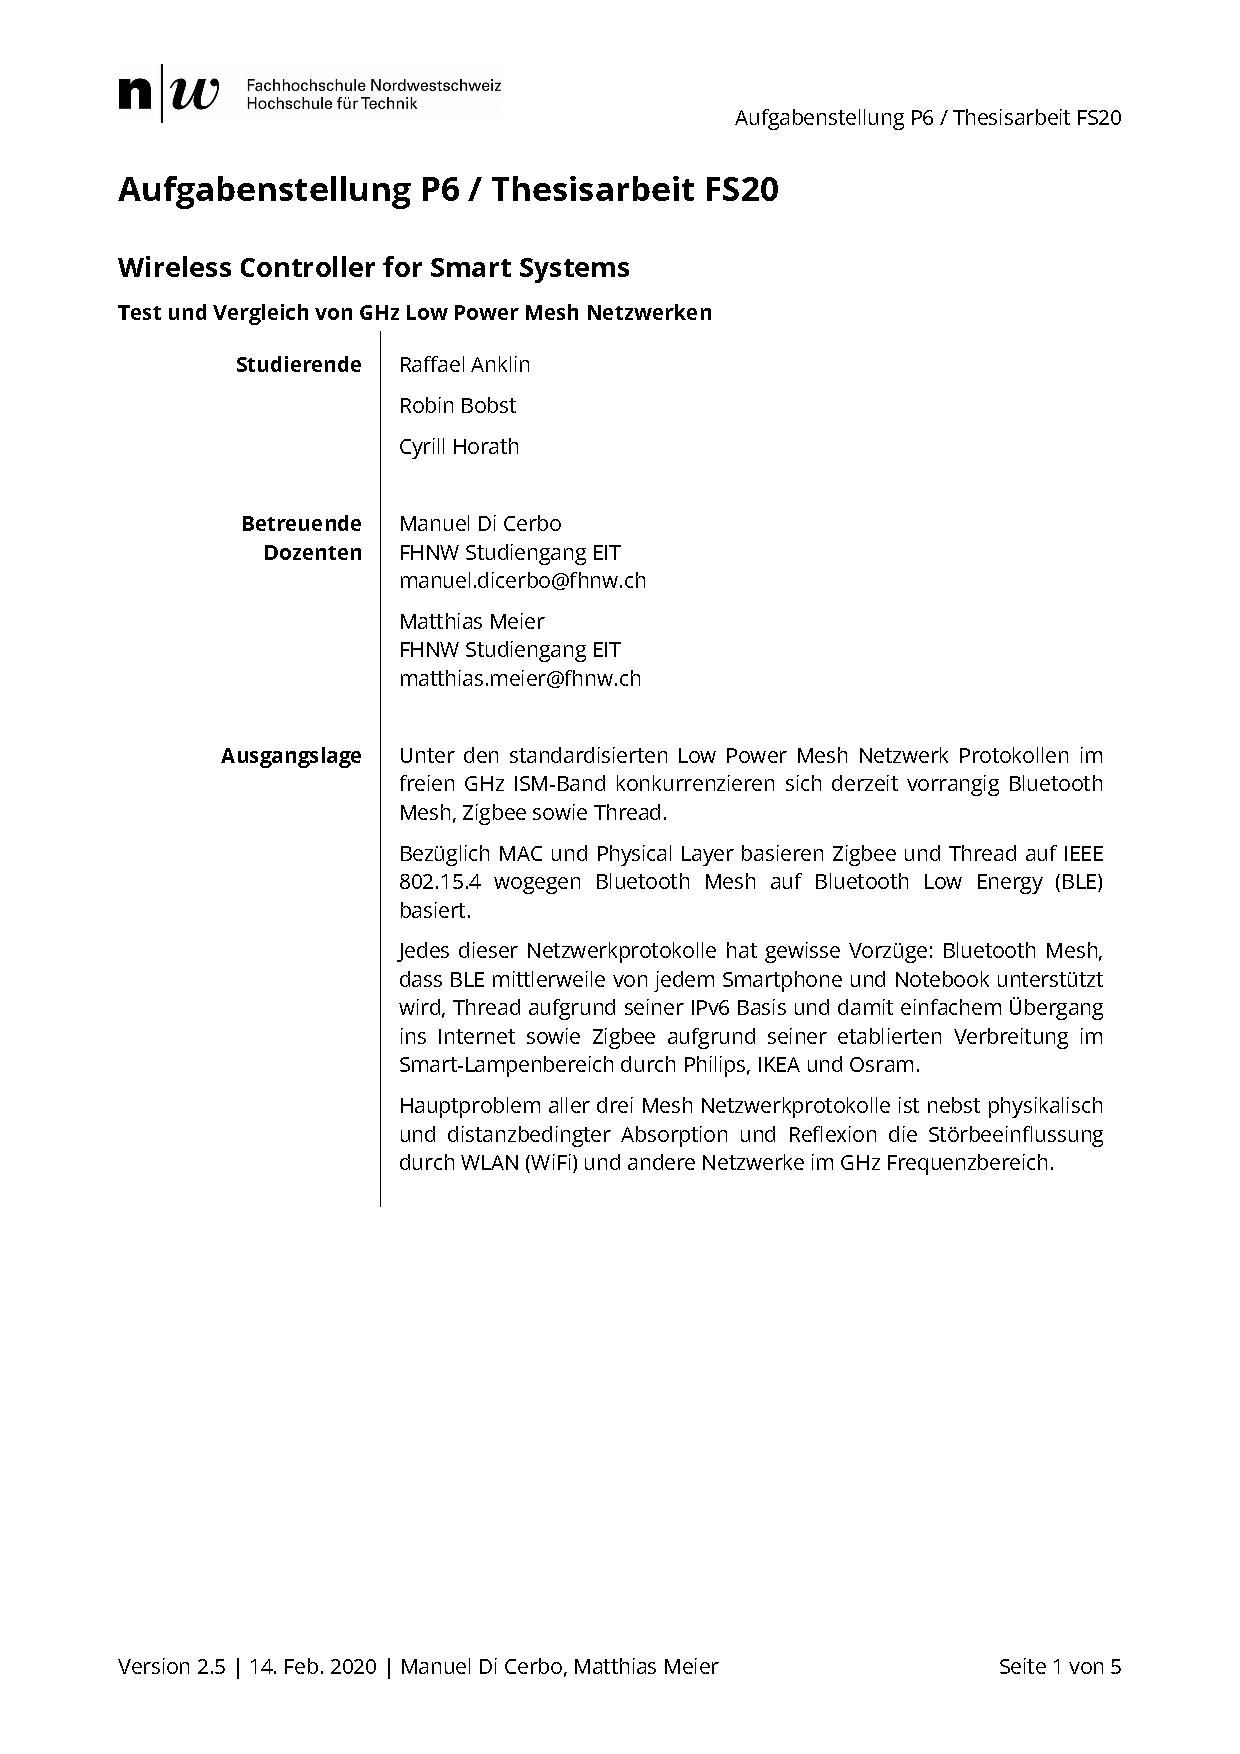
\includepdf[pages={1}, nup=1x1, landscape=false, scale=0.9 ,offset=0 -45, pagecommand={\section{Aufgabenstellung}\label{app:Aufgabenstellung}\thispagestyle{myheadings}}]{appendix/P6_Aufgabenstellung_Wireless_Controller_for_Smart_Systems.pdf}

\includepdf[pages={2-5}, nup=1x1, landscape=false, scale=0.9 ,offset=0 -45, pagecommand={\thispagestyle{myheadings}}]{appendix/P6_Aufgabenstellung_Wireless_Controller_for_Smart_Systems.pdf}


%**********************Pflichtenheft***************************

\includepdf[pages={1}, nup=1x1, landscape=false, scale=0.95 ,offset=0 -45, pagecommand={\section{Pflichtenheft}\label{app:Pflichtenheft}\thispagestyle{myheadings}}]{appendix/P6_Pflichtenheft.pdf}


\includepdf[pages={2-19}, nup=1x1, landscape=false, scale=0.95 ,offset=0 -45, pagecommand={\thispagestyle{myheadings}}]{appendix/P6_Pflichtenheft.pdf}

%***************EMV Bericht Abstrahlung Antennen*********************
\includepdf[pages={1}, nup=1x1, landscape=false, scale=0.95 ,offset=0 -45, pagecommand={\section{Bericht emv Messung Development Kits}\label{app:BerichtemvMessungDevelopmentKits}\thispagestyle{myheadings}}]{appendix/emv_Bericht_FS20.pdf}

\includepdf[pages={2-13}, nup=1x1, landscape=false, scale=0.95 ,offset=0 0, pagecommand={\thispagestyle{myheadings}}]{appendix/emv_Bericht_FS20.pdf}

%***************Messprotokolle Mesh Benchmark*********************
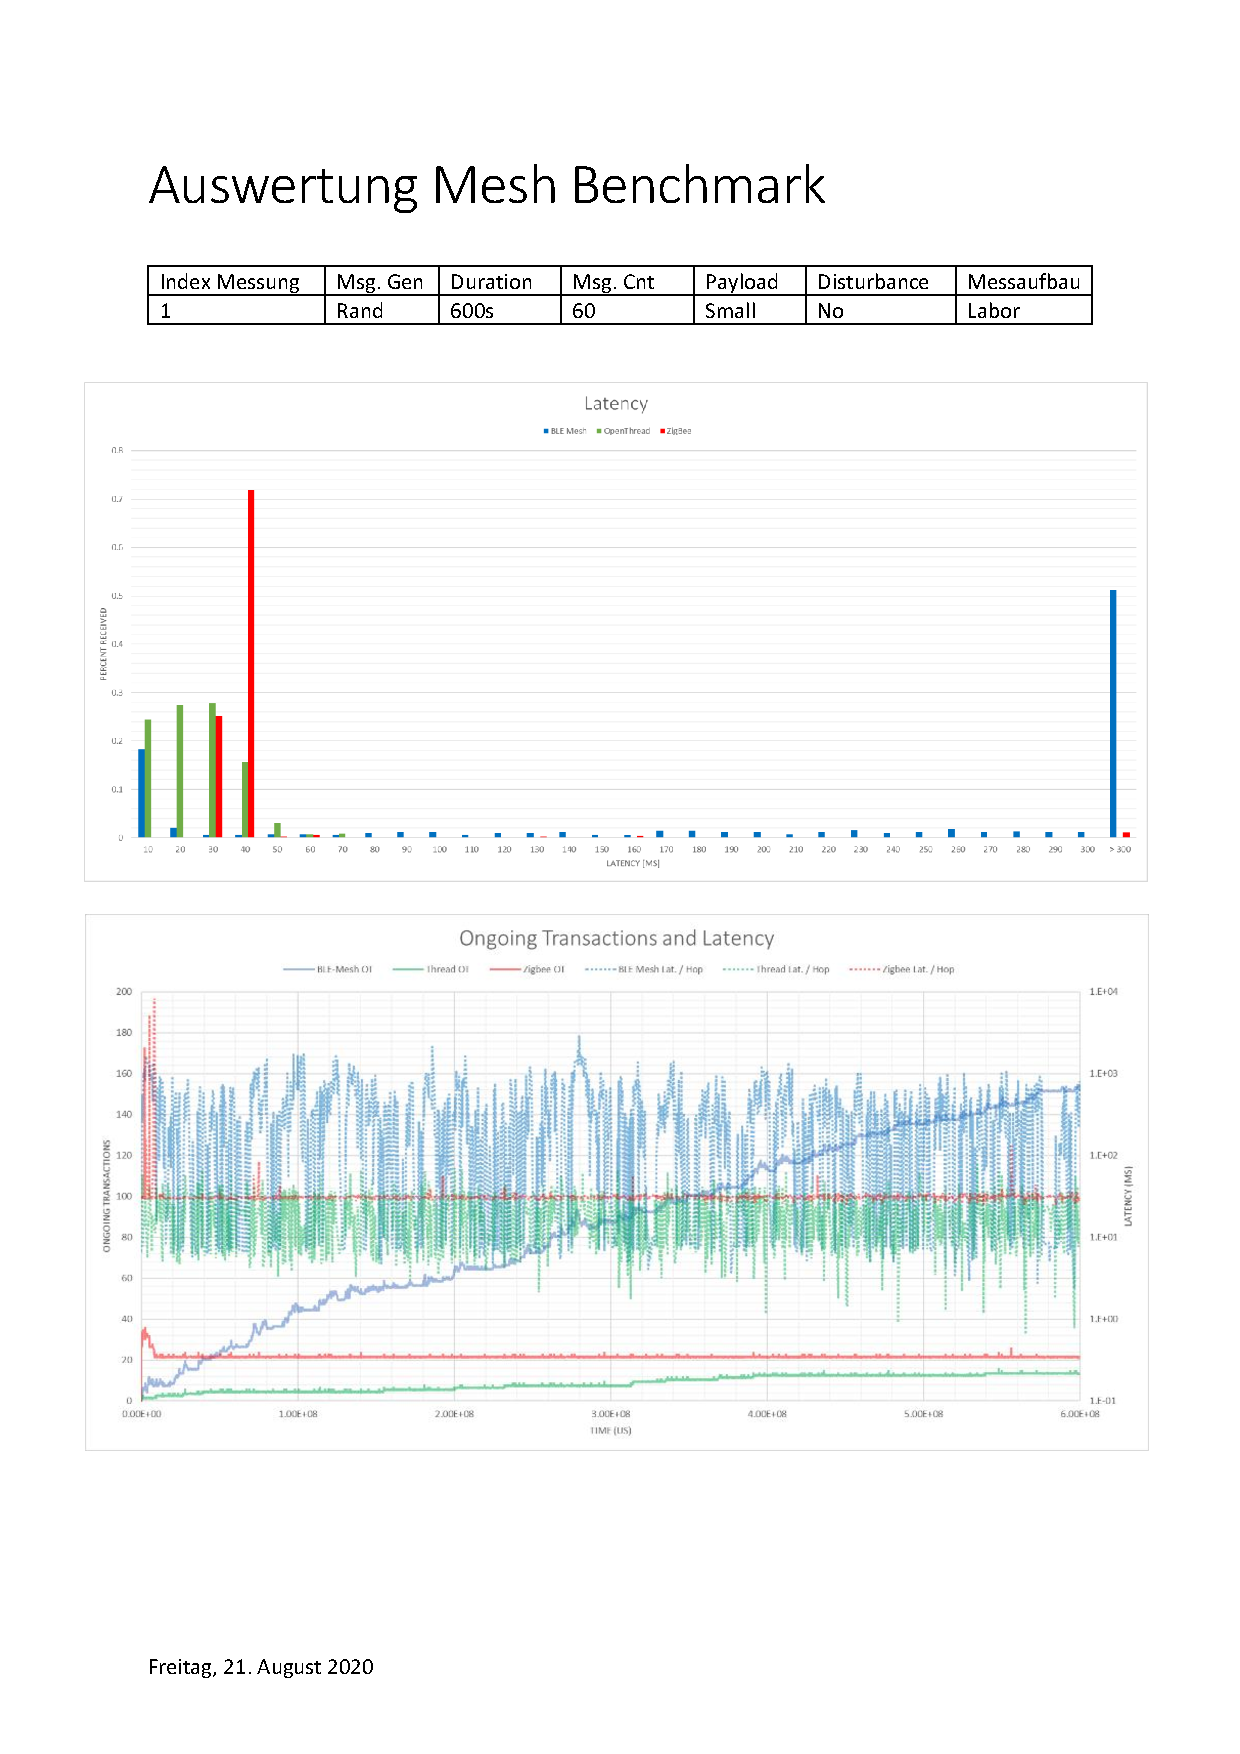
\includepdf[pages={1}, nup=1x1, landscape=false, scale=0.95 ,offset=0 -20, pagecommand={\section{Messprotokolle Mesh Benchmark}\label{app:MessprotokolleMeshBenchmark}\thispagestyle{myheadings}}]{appendix/Messprotokolle_Labor.pdf}

\includepdf[pages={2-14}, nup=1x1, landscape=false, scale=0.95 ,offset=0 0, pagecommand={\thispagestyle{myheadings}}]{appendix/Messprotokolle_Labor.pdf}

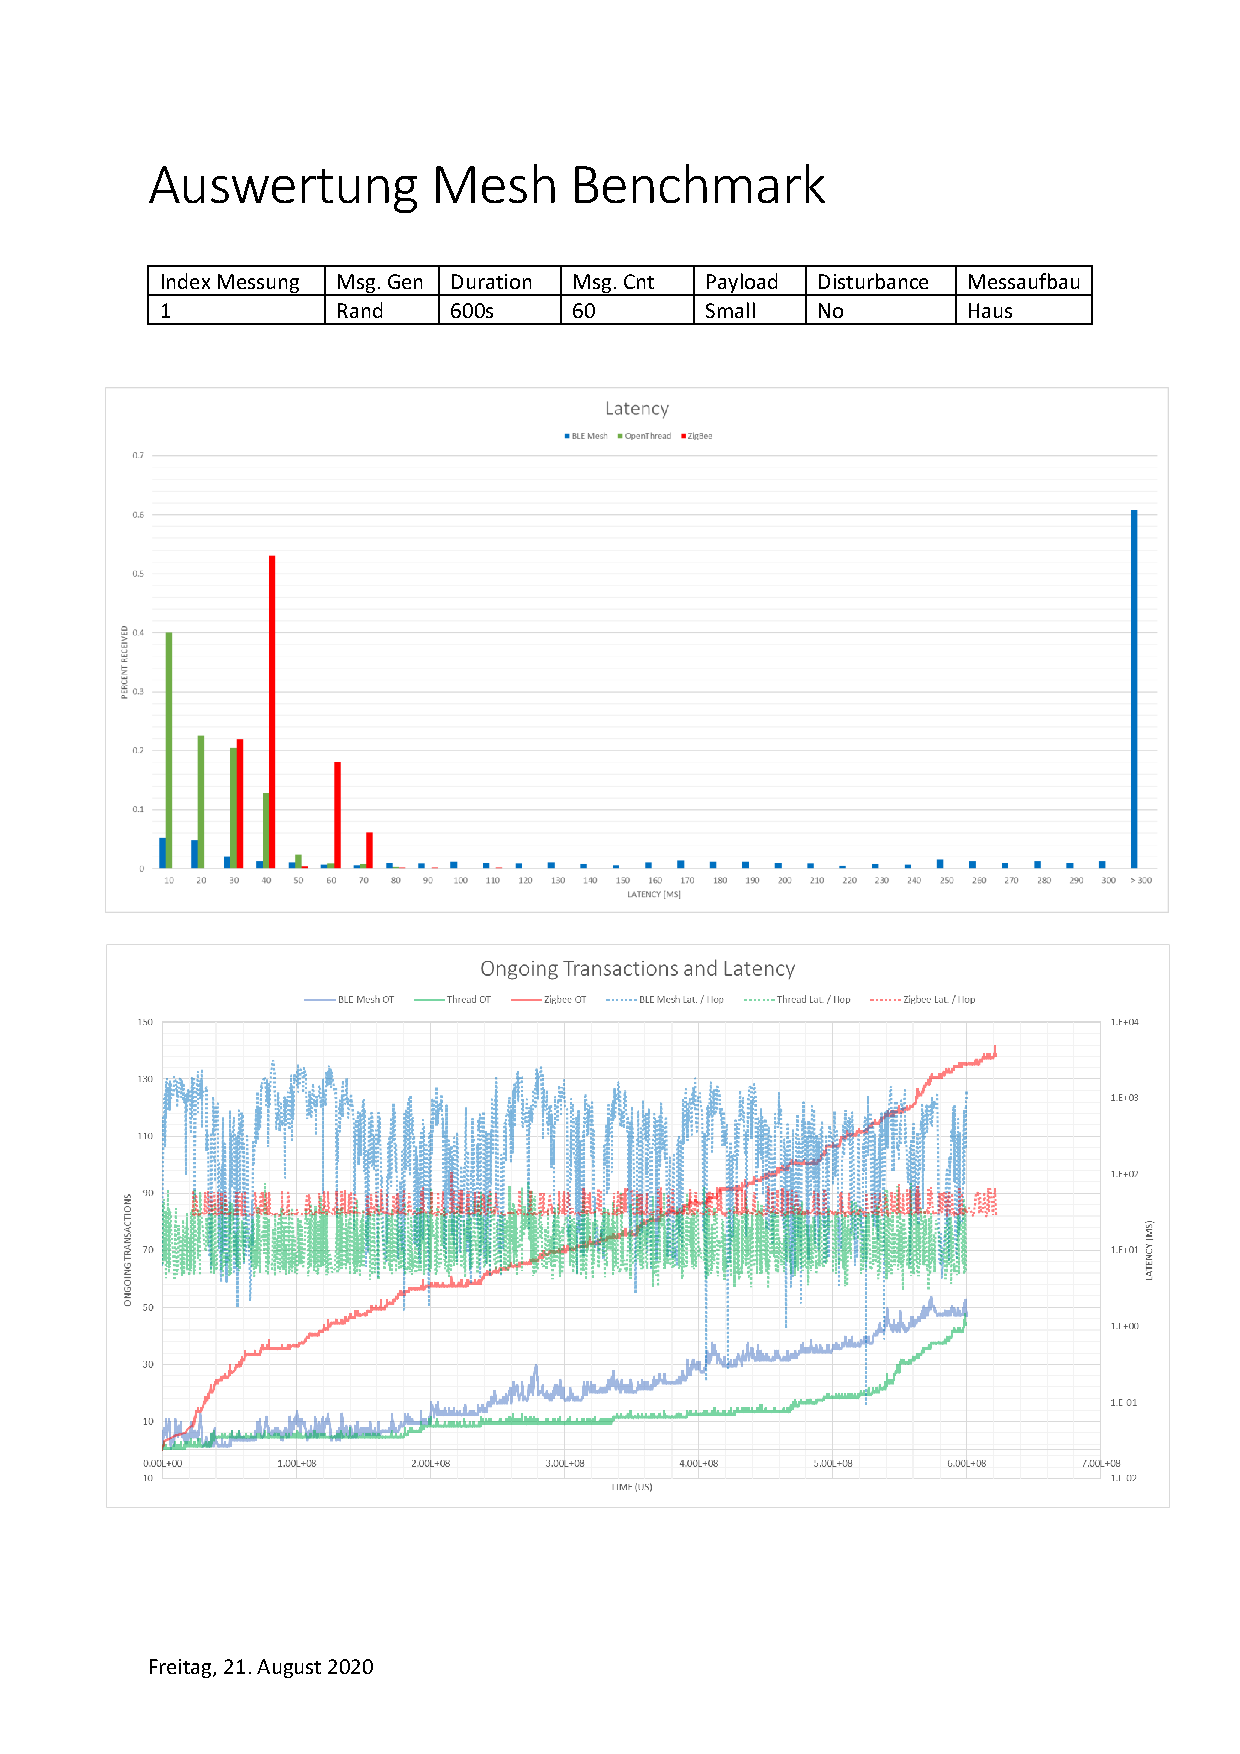
\includepdf[pages={1}, nup=1x1, landscape=false, scale=0.95 ,offset=0 0, pagecommand={\thispagestyle{myheadings}}]{appendix/Messprotokolle_Haus.pdf}

\includepdf[pages={2-8}, nup=1x1, landscape=false, scale=0.95 ,offset=0 0, pagecommand={\thispagestyle{myheadings}}]{appendix/Messprotokolle_Haus.pdf}

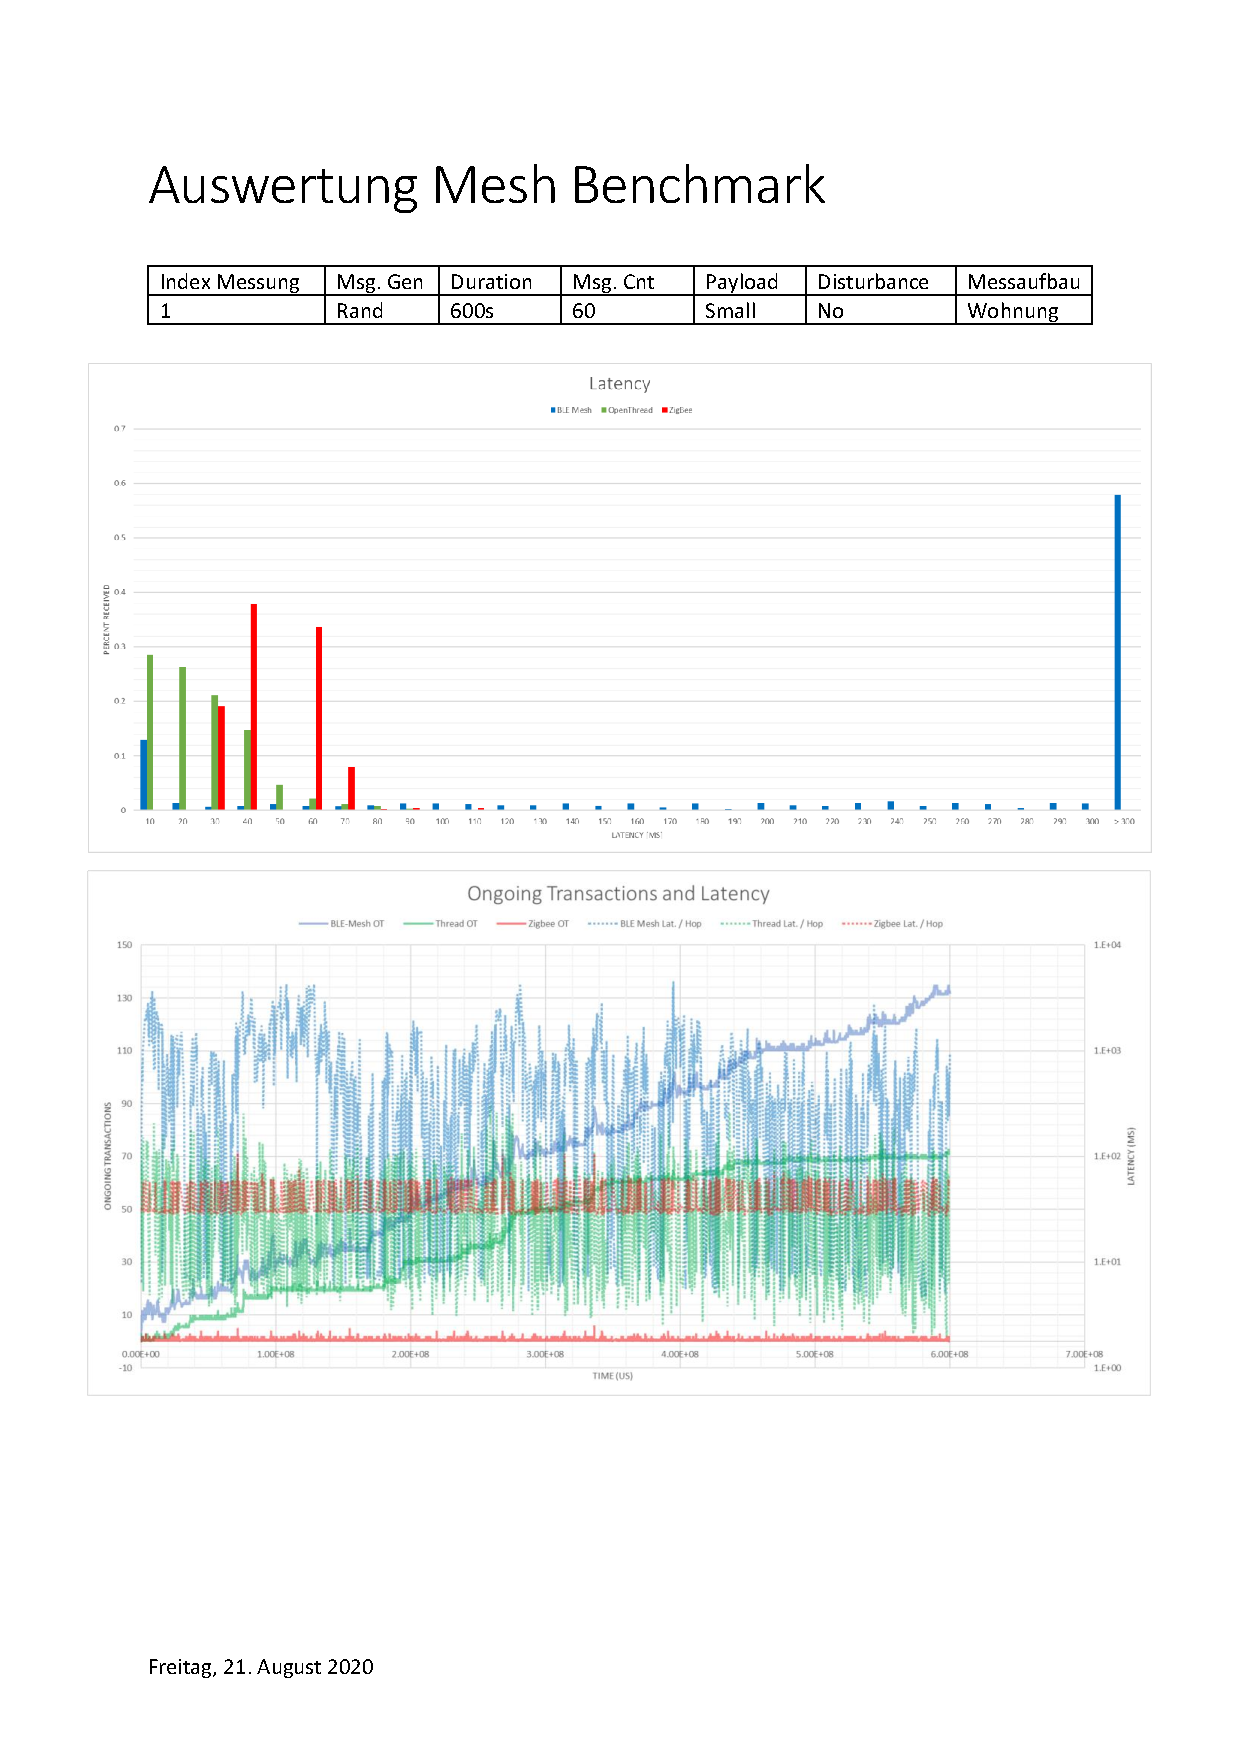
\includepdf[pages={1}, nup=1x1, landscape=false, scale=0.95 ,offset=0 0, pagecommand={\thispagestyle{myheadings}}]{appendix/Messprotokolle_Wohnung.pdf}

\includepdf[pages={2-8}, nup=1x1, landscape=false, scale=0.95 ,offset=0 0, pagecommand={\thispagestyle{myheadings}}]{appendix/Messprotokolle_Wohnung.pdf}

%***************Random Value Generation*********************
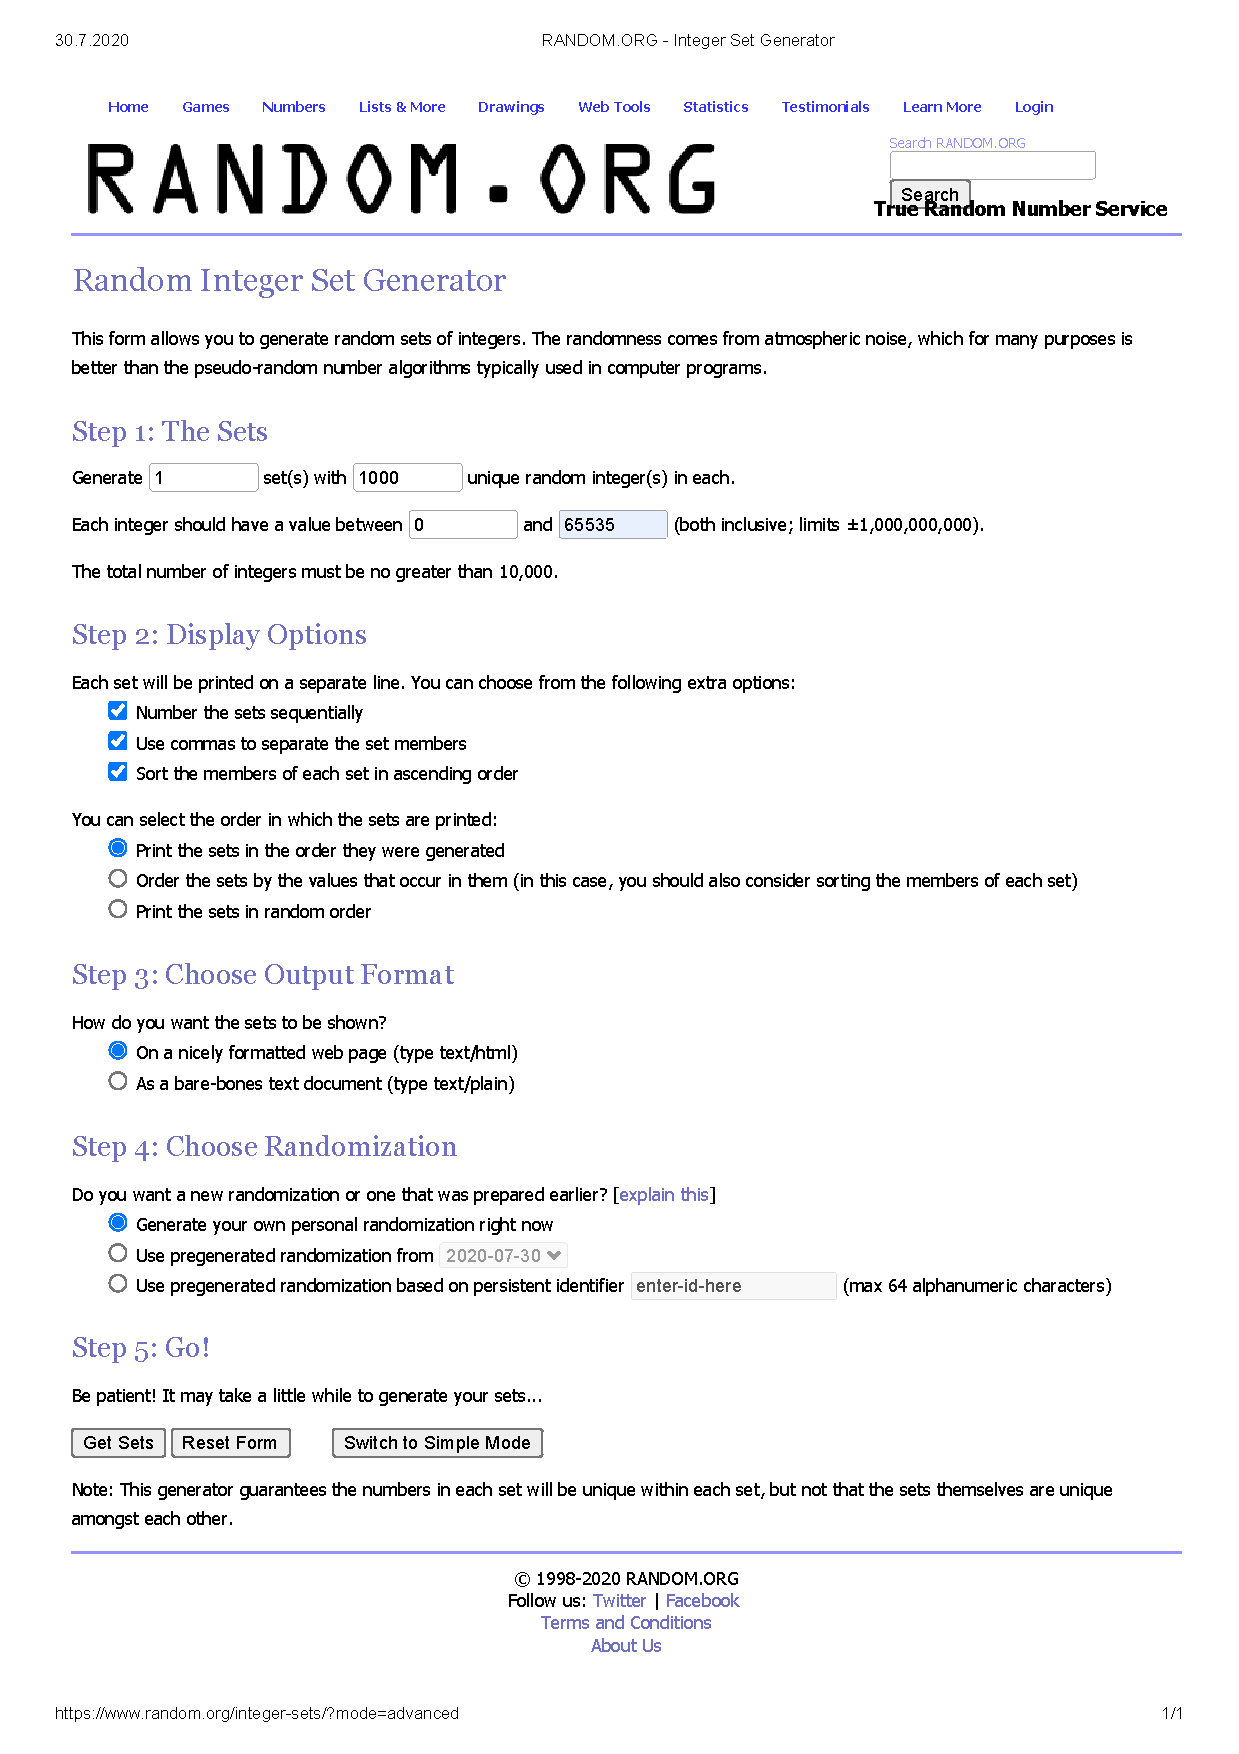
\includepdf[pages={1}, nup=1x1, landscape=false, scale=0.8 ,offset=0 -20, pagecommand={\section{Random Traffic Generation}\label{app:RandomTrafficGeneration}\thispagestyle{myheadings}}]{appendix/RANDOM.ORG_Integer_Set_Generator.pdf}


\end{appendix}



%%---NOTES for DEBUG---------------------------------------------------------------------
\ifdraft{%Do this only if mode=draft
%%requires \usepackage{todonotes})
\newpage
\listoftodos[\section{Todo-Notes}]
\clearpage
}
{%Do this only if mode=final
}

\end{document}
